\subsection{Arte con TSP}
\label{subsection:ARTTSP}
El arte con TSP son una serie de ejercicios que ponen a prueba la capacidad de los algoritmos de TSP. Se selecciona una imagen, se eligen algunos puntos y se conectan entre ellos como si fuera un problema de TSP. Según \cite{[BRIDGES]} el matemático Robert Bosch y el profesor Craig S. Kaplan presentaron este tema con una serie de imágenes que se muestran en la figura \ref{fig:EjemplosTSP.png} basadas en fotografías de Phil Greenspun.\\

     \begin{figure}[hbtp]
        \centering
            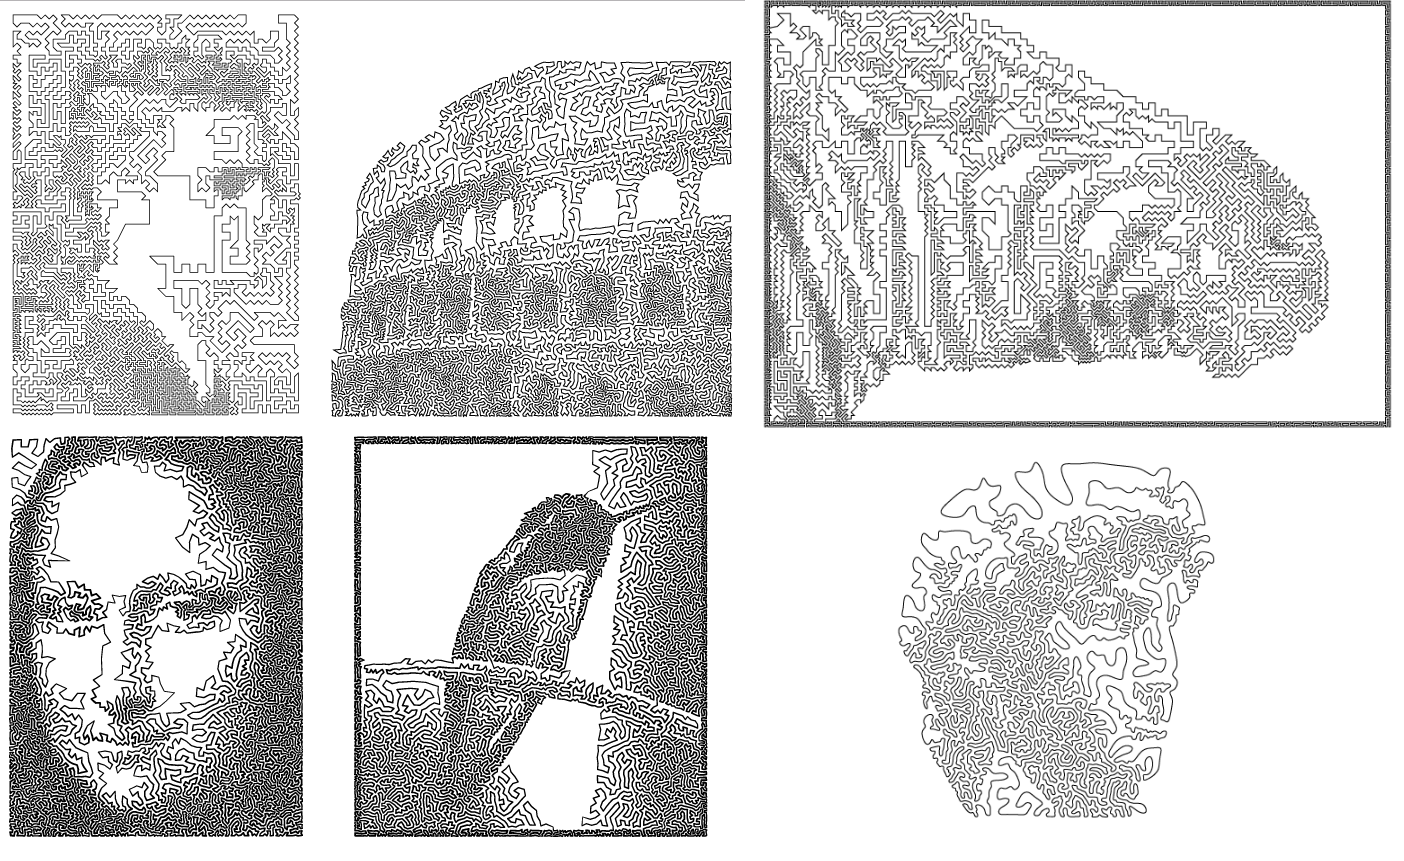
\includegraphics[width=1\textwidth]{PruebasResultados/Imagenes/EjemplosTSP.png}
            \caption{Ejemplos de arte con TSP.}
            \label{fig:EjemplosTSP.png}
    \end{figure}
    
\hspace*{1cm} Aunque no se abarcará este tema es importante señalar que se aplicó también un algoritmo que permite ver la densidad de una zona de puntos, eliminando y redistribuyendo zonas de puntos para obtener matices de blanco y negro, este método en particular fue desarrollado por Robert Bosch y Adriane Herman\\

     \begin{figure}[hbtp]
        \centering
            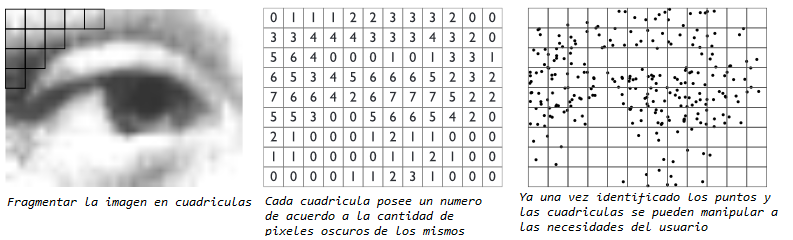
\includegraphics[width=1\textwidth]{PruebasResultados/Imagenes/BoschProceso.png}
            \caption{Breve explicación del proceso de semitonos utilizado por Bosch y Herman.}
            \label{fig:BoschProceso.png}
    \end{figure}
    
\hspace*{1cm} A continuación se presentarán algunos problemas de TSP hechos por Robert Bosch basándose en cuadros famosos, estos problemas fueron resueltos usando el método de cuadrantes sin aplicar metaheurísticas, el nombre de la pintura y el resultado se pueden ver en las mismas figuras.\\
\hspace*{1cm} También se encuentra la tabla \ref{table:tablacomparativaARTTSP} que recompila los resultados mostrados comparado con la persona que posee el record actual según \cite{[MONALISA]} cuyo nombre es Yuichi Nagata \cite{[TOKYO]}.\\

% Please add the following required packages to your document preamble:
% \usepackage[table,xcdraw]{xcolor}
% If you use beamer only pass "xcolor=table" option, i.e. \documentclass[xcolor=table]{beamer}
\begin{table}[hbtp]
\centering
\caption{Comparación con los resultados de Yuichi Nagata.}
\resizebox{1\textwidth}{!}{
\rotatebox{0}{

\begin{tabular}{llrrrr}
\hline
\rowcolor[HTML]{656565} 
\multicolumn{1}{c}{\cellcolor[HTML]{656565}{\color[HTML]{FFFFFF} \textbf{Cuadro original}}} & \multicolumn{1}{c}{\cellcolor[HTML]{656565}{\color[HTML]{FFFFFF} \textbf{Autor}}} & \multicolumn{1}{c}{\cellcolor[HTML]{656565}{\color[HTML]{FFFFFF} \textbf{Ciudades}}} & \multicolumn{1}{c}{\cellcolor[HTML]{656565}{\color[HTML]{FFFFFF} \textbf{Record actual}}} & \multicolumn{1}{c}{\cellcolor[HTML]{656565}{\color[HTML]{FFFFFF} \textbf{Cuadrantes}}} & \multicolumn{1}{c}{\cellcolor[HTML]{656565}{\color[HTML]{FFFFFF} \textbf{Diferencia (\%)}}} \\ \hline
Mona Lisa                                                                                   & Leonardo Da Vinci                                                                  & 100,000                                                                            & 5,757,191                                                                                & 6,471,018                                                                                & 12.39                                                                                     \\ \hline
Auto retrato                                                               					& Vincent Van Gogh                                                                   & 120,000                                                                            & 6,543,610                                                                                & 7,401,998                                                                                & 13.11                                                                                     \\ \hline
El nacimiento de Venus                                                                      & Sandro Botticelli                                                                  & 140,000                                                                            & 6,810,665                                                                                & 7,653,034                                                                                & 12.36                                                                                     \\ \hline
Juan de Pareja                                                                  			& Diego Velázquez                                                                    & 160,000                                                                            & 7,619,953                                                                                & 8,586,457                                                                                & 12.68                                                                                     \\ \hline
El desesperado                                                                              & Gustave Courbet                                                                    & 180,000                                                                            & 7,888,733                                                                                & 8,951,892                                                                                & 13.47                                                                                     \\ \hline
La joven de la perla                                                         				& Johannes Vermeer                                                                   & 200,000                                                                            & 8,171,677                                                                                & 9,357,118                                                                                & 14.50                                                                                     \\ \hline
\end{tabular}
}
}
\label{table:tablacomparativaARTTSP}
\end{table} 

\clearpage \newpage
      
    \begin{figure}[hbtp]
        \centering
            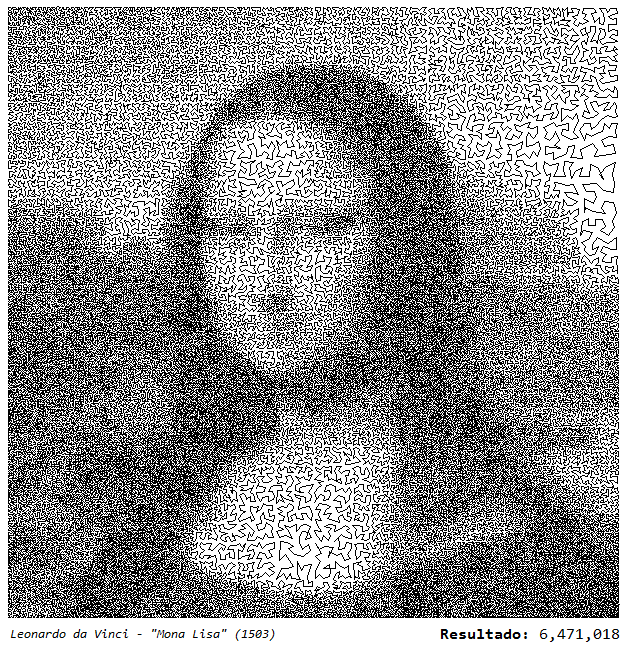
\includegraphics[width=1\textwidth]{PruebasResultados/Imagenes/TSP_ART/monalisatsp.png}
            \caption{"Mona Lisa" de Leonardo Da Vinci hecho en TSP.}
            \label{fig:monalisatsp.png}
    \end{figure}
      \clearpage \newpage  
      
    \begin{figure}[hbtp]
        \centering
            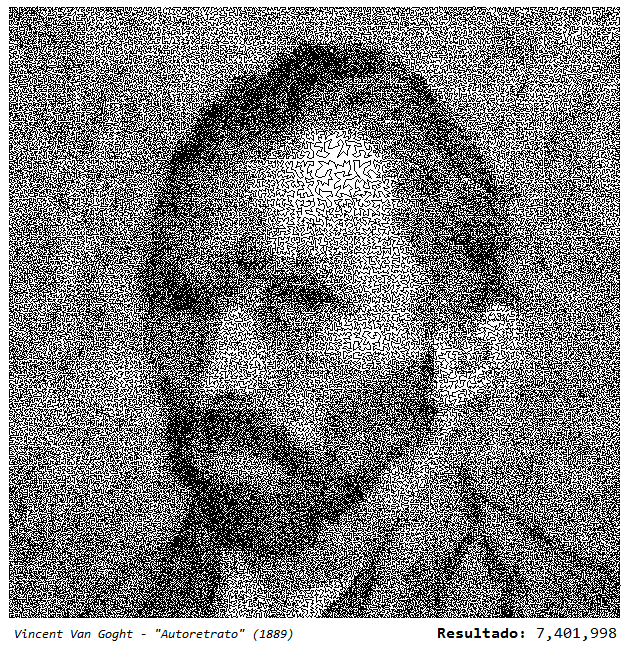
\includegraphics[width=1\textwidth]{PruebasResultados/Imagenes/TSP_ART/vangogh.png}
            \caption{"Autoretrato" de Vincent Van Gogh hecho en TSP.}
            \label{fig:vangogh.png}
    \end{figure}
      \clearpage \newpage  
      
    \begin{figure}[hbtp]
        \centering
            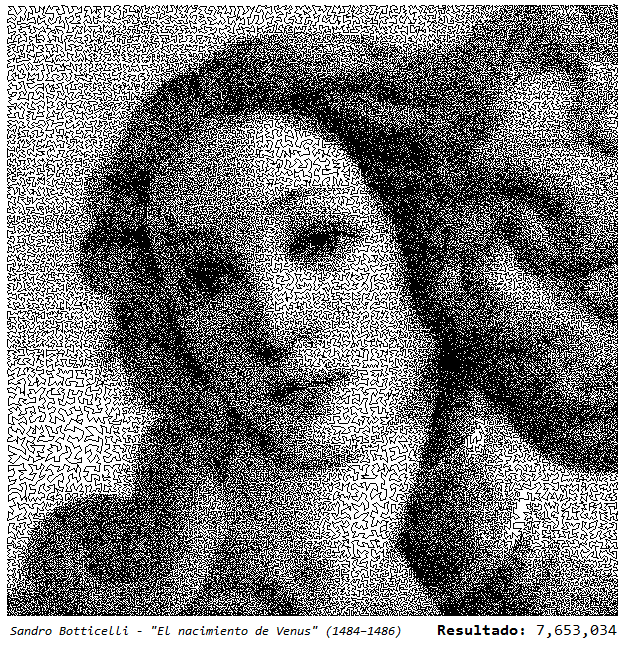
\includegraphics[width=1\textwidth]{PruebasResultados/Imagenes/TSP_ART/Venus.png}
            \caption{"El nacimiento de Venus" de Sandro Botticelli hecho en TSP.}
            \label{fig:Venus.png}
    \end{figure}
      \clearpage \newpage  
      
    \begin{figure}[hbtp]
        \centering
            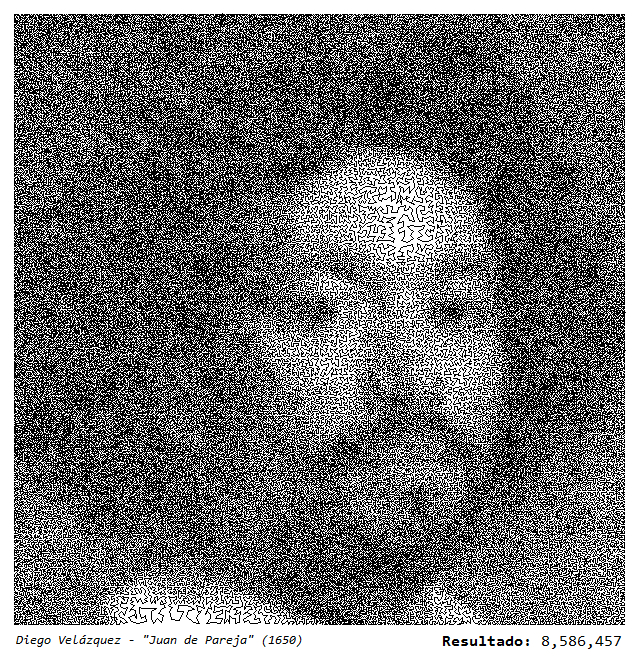
\includegraphics[width=1\textwidth]{PruebasResultados/Imagenes/TSP_ART/pareja.png}
            \caption{"Juan de Pareja" de Diego Velázquez hecho en TSP.}
            \label{fig:pareja.png}
    \end{figure}
      \clearpage \newpage   
      
     \begin{figure}[hbtp]
        \centering
            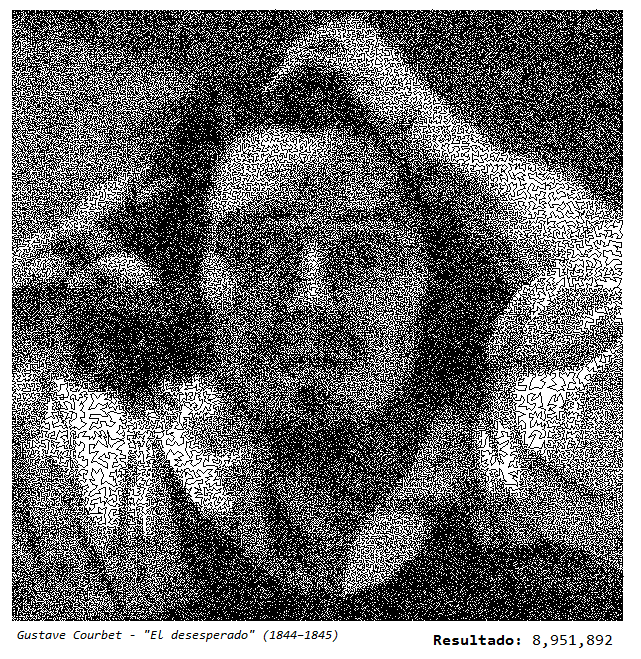
\includegraphics[width=1\textwidth]{PruebasResultados/Imagenes/TSP_ART/courbet.png}
            \caption{"El desesperado" de Gustave Courbet hecho en TSP.}
            \label{fig:courbet.png}
    \end{figure}
      \clearpage \newpage
      
    \begin{figure}[hbtp]
        \centering
            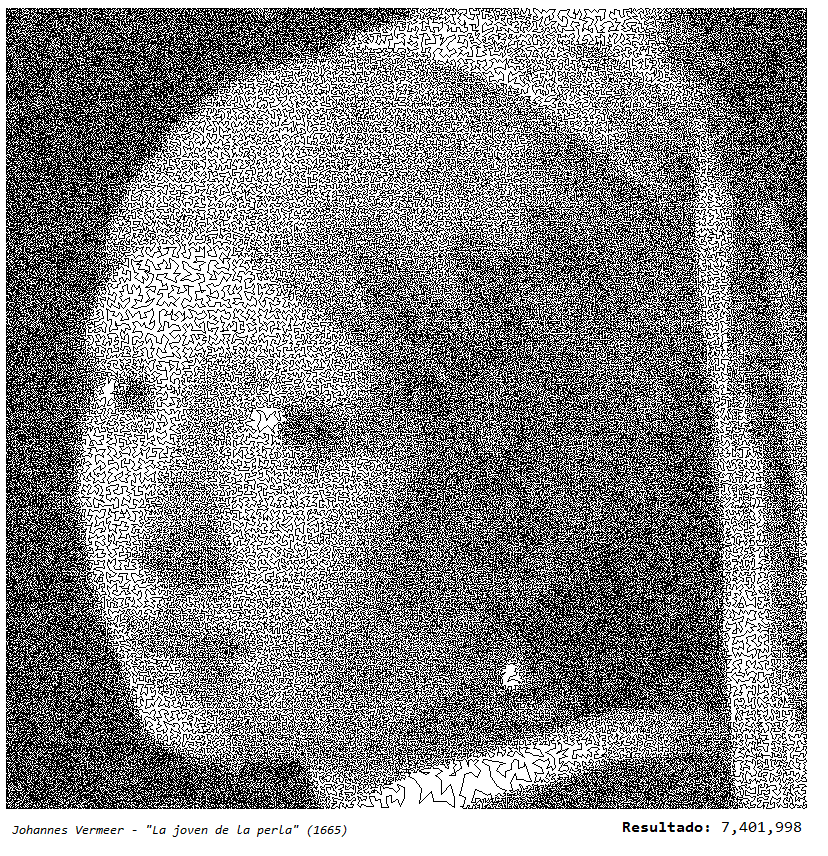
\includegraphics[width=1\textwidth]{PruebasResultados/Imagenes/TSP_ART/earring.png}
            \caption{"La joven de la perla" de Johannes Vermeer hecho en TSP.}
            \label{fig:earring.png}
    \end{figure}
      \clearpage \newpage